\documentclass[output=paper]{LSP/langsci}  
\author{Christoph Wolk\affiliation{?} \lastand Benedikt Szmrecsanyi\affiliation{?}}
\title{Top-down and bottom-up advances in corpus-based dialectometry}
\abstract{We present three approaches to corpus-based dialectometry and apply them to morphosyntactic variation in the \emph{Freiburg Corpus of English Dialects}, which covers 34 counties throughout Great Britain.
Two of these are \emph{top-down approaches} that start with a predefined feature list; one using a straightforward frequency-based analysis, the other enhancing the raw numbers using probabilistic modeling.
Both methods are able to detect the structure of areal variation in Great Britain, and the second approach is able to reduce the influence of textual coverage as a nuisance factor.
The final approach is a \emph{bottom-up} method that eschews pre-specified lists and evaluates potential features directly from the data using a permutation-based metric.
Again, we find that simple frequency-based metrics are biased, but that derived metrics yield a clearer pattern.
Using these methods, we are able to uncover significant geolinguistic structure in Great Britain.
}

\maketitle 
\begin{document}
  

\section{Introduction}

\il{British English|(}
In this contribution, we sketch novel ways to conduct dialectometry. Let us set the scene by fixing some terminology first. \textsc{Linguistic corpora} are principled and broadly representative collections of naturalistic texts or speech. Linguistic corpora thus sample \textsc{usage data}, and as such are increasingly popular in dialectology (\citealt{anderwald_corpus_2009,grieve_corpus-based_2009}) and beyond (see the papers in \citealt{szmrecsanyi_aggregating_2014}). \textsc{corpus linguistics}, accordingly, is a methodology in linguistics that bases claims about language on corpora. Corpus linguistics is thus the methodological outgrowth of the usage-based turn in linguistics, in the spirit of, e.g.,  \citet{bybee_language_2010,tomasello_constructing_2003}. As is well known, \textsc{classical dialectometry} in the tradition of \citet{goebl_dialektometrische_1984,nerbonne_edit_1999} draws on atlas material to explore geolinguistic patterns using aggregation methodologies. By contrast, \textsc{corpus-based dialectometry} (henceforth: \textsc{cbdm}) utilizes aggregation methodologies to explore quantitative and distributional usage patterns extracted from dialect corpora.

Why do we need \textsc{cbdm}? 
After all, there is some scepticism in the community about the usefulness of non-atlas resources (\citealt[499]{goebl_dialektometrie_2005}, for example, writes that ``Extra atlantes linguisticos nulla salus dialectometrica'').
Let us emphasize first that we do not wish to suggest that linguistic atlases are dispensable. 
Quite on the contrary, we are convinced that they are quite indispensable for some purposes, such as surveying -- from a bird's eye perspective -- the variable presence or absence of particular features in particular language or dialect areas.
But at the same time we believe that also (!) being able to analyze naturalistic corpus data is central to the maturation of the dialectometry enterprise.
The reason is that the data in (most) linguistic atlases speak primarily to the issue of explicit, active linguistic knowledge, while corpus data document first and foremost usage (which is, of course, related to knowledge of the more implicit sort, but there is no 1-1 correspondence).
Thus turning to corpora will enable dialectologists to address hitherto rather neglected questions about usage versus knowledge,  production/comprehension versus intuition, chaos versus orderliness, and so on. 
We should also add that neighboring linguistic disciplines, such as variationist sociolinguistics, rely empirically almost exclusively on usage data. 
It is precisely because of this that there is some welcome methodological convergence to be had in the field. 
The disadvantage of \textsc{cbdm} is that corpus methodologies are not well suited to study low-frequency phenomena; rare things, in other words, are better investigated drawing on atlases and surveys.

In this contribution we sketch three \textsc{cbdm} approaches, two top-down, the third bottom-up. The top-down approaches first define a feature catalogue, then establish the frequencies and/or probabilities associated with the features, and finally aggregate over them. The bottom-up approach, by contrast, lets the features to be aggregated emerge in a data-driven fashion through the identification of significant and/or distinctive part-of-speech \emph{n}-grams. The case studies which we present to illustrate these approaches summarize work by \citet{szmrecsanyi_grammatical_2013} and \citet{wolk_integrating_2014}. All case studies are concerned with grammatical variation in traditional British English dialects.

This contribution is structured as follows. In Section \ref{FRED} we sketch the dialect corpus into which we tap. Section \ref{topdown} describes the top-down \textsc{cbdm} approach; Section \ref{bottomup} is dedicated to the bottom-up approach. Section \ref{conclusion} offers some concluding remarks.


\section{The Freiburg Corpus of English Dialects (FRED)}\label{FRED}

The case studies in this contribution will analyze the \emph{Freiburg Corpus of English Dialects} (henceforth: \textsc{fred}) (see \citealt{hernandez_users_2006} for details). 
The version of the corpus used in the top-down \textsc{cbdm} study (Section \ref{topdown}) contains 368 individual texts and covers approximately 2.44 million words of running text (this corresponds to about 300 hours of speech), mainly transcribed so-called `oral history' material. 
These were mostly recorded between 1970 and 1990. 
The typical setting is that a fieldworker interviews an informant about life, work, etc. in the olden days. 
The 431 informants represented in the corpus are typically elderly people with a working-class background -- so-called \textsc{norm}s (\emph{non-mobile old rural males}) (cf. \citealt[29]{chambers_dialectology_1998}). 
The interviews were conducted in 156 different locations -- that is, villages and towns -- in 34 different pre-1974 counties in Great Britain including the Isle of Man and the Hebrides. These counties are displayed in Figure \ref{coverage}. 
Note that we aggregate all texts/interviews from the same county, in order to obtain 34 distinct subcorpora.
Individual texts are annotated with longitude/latitude information; county coordinates (mean longitude and latitude) have consequently been calculated by computing the arithmetic mean of all the location coordinates associated with a particular county. 
Some of the informants had to be removed for the analysis presented in Section \ref{sec:prob} due to missing metadata.
This led to the complete removal of three counties for that analysis: East Lothian, Denbighshire and Warwickshire.

%%%%%%%%%%%%%%%%%%%%%%%%%%%%%%%%%%%%%%%%%%%%%%%%%%%%%%%%%%%%%%%%%%%%%%%%%%%%%%%%%%%%%%%%%%%%%%%%%%%%%%%%%%%%%%%%%%%%%%%%%%%%%%%
\begin{figure}[t]
    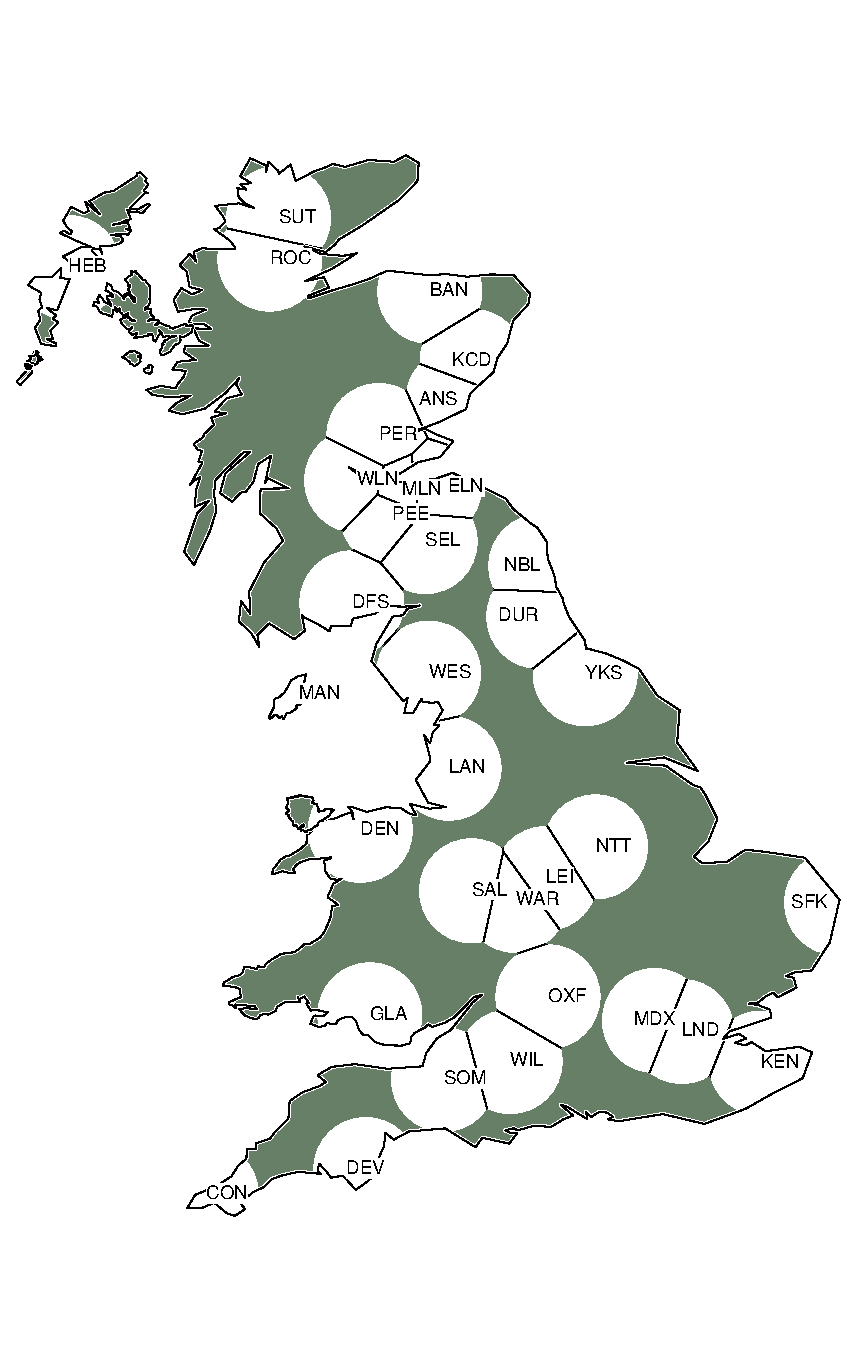
\includegraphics [keepaspectratio,width=.5\textwidth] {illustrations/wolk_map_descr_all34_counties.eps}
    \caption{Pre-1974 counties represented in \textsc{fred}. See \url{http://en.wikipedia.org/wiki/Chapman_code} for an explanation of the county codes.}\label{coverage}
\end{figure}

%%%%%%%%%%%%%%%%%%%%%%%%%%%%%%%%%%%%%%%%%%%%%%%%%%%%%%%%%%%%%%%%%%%%%%%%%%%%%%%%%%%%%%%%%%%%%%%%%%%%%%%%%%%%%%%%%%%%%%%%%%%%%%%

In the bottom-up \textsc{cbdm} study (Section \ref{bottomup}), we will analyze a smaller version of the corpus: the Freiburg Corpus of English Dialects Sampler (\textsc{fred-s}) (\citealt{szmrecsanyi_manual_2007}). \textsc{fred-s} contains a subset of the texts in the full \textsc{fred} corpus totaling about 1 million words of running text and covering 17 counties in England the Scottish Lowlands. The big advantage of using \textsc{fred-s}, though smaller in size, is that it exists in a version that was automatically part-of-speech (\textsc{pos}) annotated by the \textsc{claws4} tagger \citep{garside_hybrid_1997} using the detailed \textsc{claws7} tagset.

To illustrate the nature of the material sampled in \textsc{fred} and \textsc{fred-s}, (\ref{FREDexample}) is the beginning of an interview conducted in 1978 in St. Ives, Cornwall (\textsc{fred} text \textsc{con}003). The informant is an 86-year old male (`CAVA\_PV'), who is interviewed by two interviewers (`IntRS' and `Inf'). Interviewer utterances are enclosed in curly brackets (note that interviewer utterances are excluded from analysis in the present study).
%%%
%%% can't get the example to italicise
%%%
\begin{exe}
\ex \label{FREDexample} \textit{\{$<$u IntRS$>$ Well you're a St. Ives man. Where were you born?\}
\newline$<$u CAVA\_PV$>$ Born Belyars Lane, eighteen ninety-two. Eighteenth of December. Worn sovereign in the cupper. Born sovereign. The poor times then, you know (gap 'indistinct') boiling potatoes and t -- inkle mosses.
\newline\{$<$u IntRS$>$ Did you, did you, how long did you live there?\}
\newline$<$u CAVA\_PV$>$ Oh we lived there about, oh about twelve years, I suppose. Then we went up to a Rosewall Terrace. Hmm. So everything's altered now to what er was then, I mean.}
%\newline\{$<$u IntRS$>$ Mhm.\}
%\newline\{$<$u Inf$>$ And you live on Baronon Hill?\}
%\newline$<$u CAVA\_PV$>$ On Baronon Hill, for a few years, uhuh. And I was only thinking here this afternoon about when we live in them Baronon Hill, you know. 'Course the back of the, the back of the castles, (gap 'mumbling') -- I don't know whether you could in there or no, I don't much, but uh, (v 'laughter') I can remember, course she was \dots put to bed. We used to live right opposite [\dots]
\end{exe}

\section{Top-down CBDM} \label{topdown}

This section will discuss top-down \textsc{cbdm}, which consists of five steps:

  \begin{description}

    \item[Step 1:] define the feature catalogue (motto: the more features, the merrier).

    \item[Step 2:] identify features in the corpus texts (automatically, semi-automatically, or manually).

    \item[Step 3:] establish raw feature frequencies (per location); subsequently, normalize frequencies and/or model frequencies probabilistically.

    \item[Step 4:] aggregate: calculate a distance matrix.

    \item[Step 5:] project to geography, analyze \& interpret.

  \end{description}

\citet{szmrecsanyi_grammatical_2013} and \citet{wolk_integrating_2014} discuss the method in meticulous detail.
Suffice it to say here that the feature catalogue we used to explore grammatical variation in British English dialects consists of $p = 57$ features, which cover all major domains in English grammar as well as the usual suspects in the variationist and dialectological literature, such as non-standard past tense \textit{done} (e.g., \textit{you came home and done the home fishing}), multiple negation (e.g., \textit{don't you make no damn mistake}), and \textit{don't} with third person singular subjects (e.g., \textit{if this man don't come up to it}).
These features were identified in the corpus material (automatically, semi-automatically, or manually -- depending on the nature of the feature), and their usage frequency established.
Subsequently, this information was arranged in an $n$ by $p$ table: $34$ counties, each characterized by a vector of $57$ feature frequencies. At this point, there are two ways to proceed: the \emph{normalization-based top-down \textsc{cbdm} approach}, pursued in \citet{szmrecsanyi_grammatical_2013}, and the \emph{probabilistically enhanced top-down \textsc{cbdm} approach}, explored in \citet{wolk_integrating_2014}.
We will now discuss these top-down variants in turn.


\subsection{The normalization-based top-down \textsc{cbdm} approach}\label{topdownnormalized}

\citet{szmrecsanyi_grammatical_2013} processed the frequency table in two ways prior to analysis. For one thing, he normalized raw frequencies to frequency per 10,000 words, doing justice to the fact that textual coverage of individual dialects varies. This normalized frequency table tells us, for example, that multiple negation is twice as frequent in Nottinghamshire than in Yorkshire. Additionally, \citeauthor{szmrecsanyi_grammatical_2013} applied a log-transformation to the normalized frequencies for the sake of de-emphasizing large frequency differentials and thus alleviating the effect of frequency outliers. Next \citeauthor{szmrecsanyi_grammatical_2013} converted the normalized, log-transformed frequency table into an $N$ by $N$ distance matrix. This transformation is an aggregation step, in that the resulting distance matrix abstracts away from individual feature frequencies and specifies pairwise distances between the objects considered. To calculate dialectal distances, \citeauthor{szmrecsanyi_grammatical_2013} used the well-known Euclidean Distance Measure (see, e.g., \citealt[25]{aldenderfer_cluster_1984}). The Euclidean Distance Measure defines the distance between two dialects as the square root of the sum of all $p$ squared frequency differentials.

Distance matrices are the customary input to dialectometric analysis and visualization techniques. Let us now explore the normalization-based top-down distance matrix using a particularly popular dialectometric mapping technique, \emph{cluster maps}. Cluster maps are common in all strands of dialectometry, and project the outcome of cluster analysis to geography (cf., for example, \citealt[Map 18]{goebl_bunch_2007}; \citealt[Figure 5]{nerbonne_dialektklassifikation_2005}; \citealt[Figure 9.6]{heeringa_measuring_2004}). First, an $N$ by $N$ distance matrix is subjected to \textsc{hierarchical agglomerative cluster analysis} (cf. \citealt{jain_data_1999}; we specifically used Ward's method as clustering algorithm), a statistical technique used to group a number of objects (in this study, dialects) into a smaller number of discrete clusters.\footnote{Simple clustering can be unstable, so we used the ``clustering with noise'' technique (\citealt{nerbonne_projecting_2008}).} Cluster memberships of dialect locations can then be projected to geography via, e.g., color coding.


%%%%%%%%%%%%%%%%%%%%%%%%%%%%%%%%%%%%%%%%%%%%%%%%%%%%%%%%%%%%%%%%%%%%%%%%%%%%%%%%%%%%%%%%%%%%%%%%%%%%%%%%%%%%%%%%%%%%%%%%%%%%%%%
\begin{sidewaysfigure} [tbp]
\begin{minipage}[b]{0.30\linewidth} % A minipage that covers half the page
    \centering
    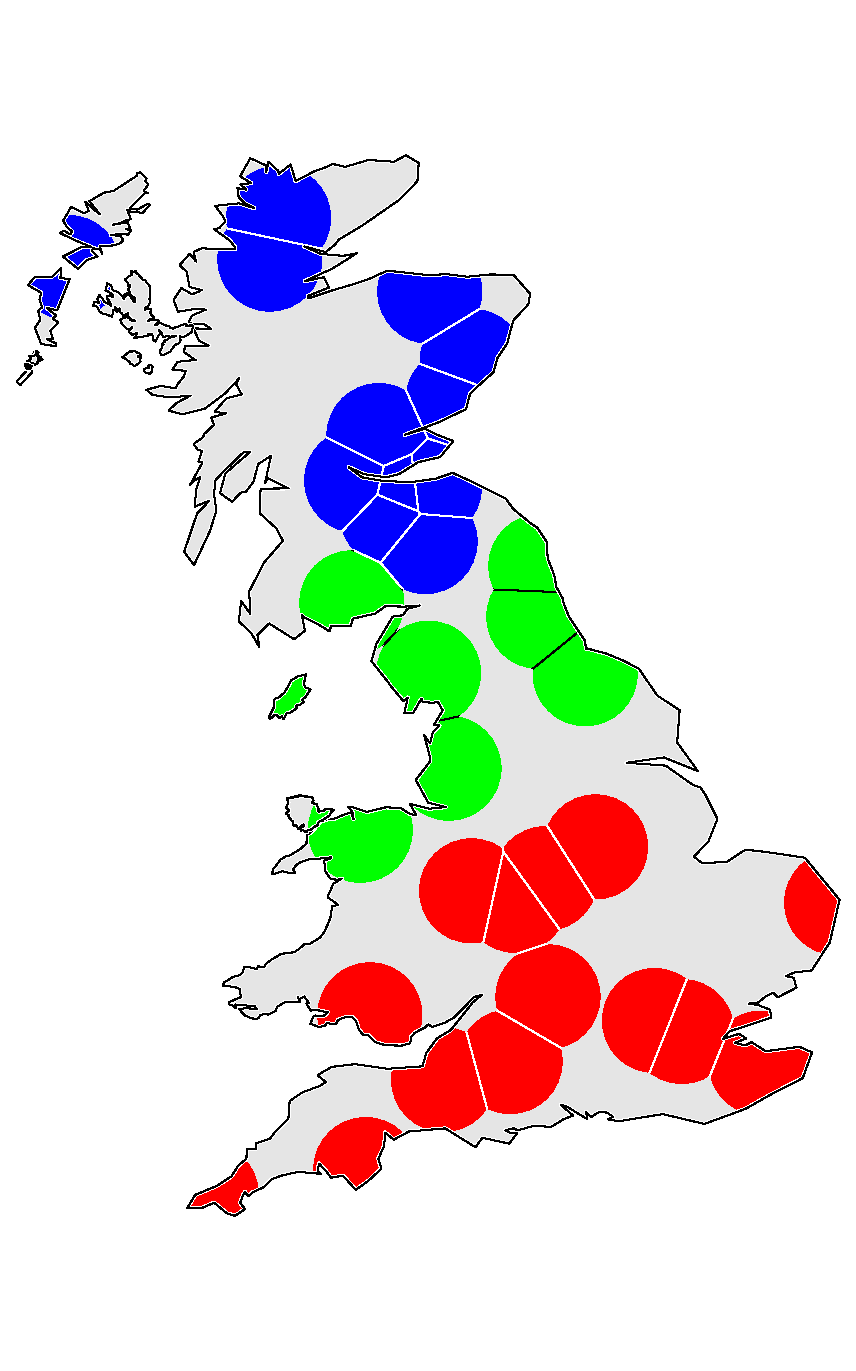
\includegraphics [keepaspectratio,width=.98\textwidth] {illustrations/wolk_WARD_crowdist_hard.eps}
\end{minipage}
\hspace{0.5cm} % To get a little bit of space between the figures
\begin{minipage}[b]{0.30\linewidth}
    \centering
    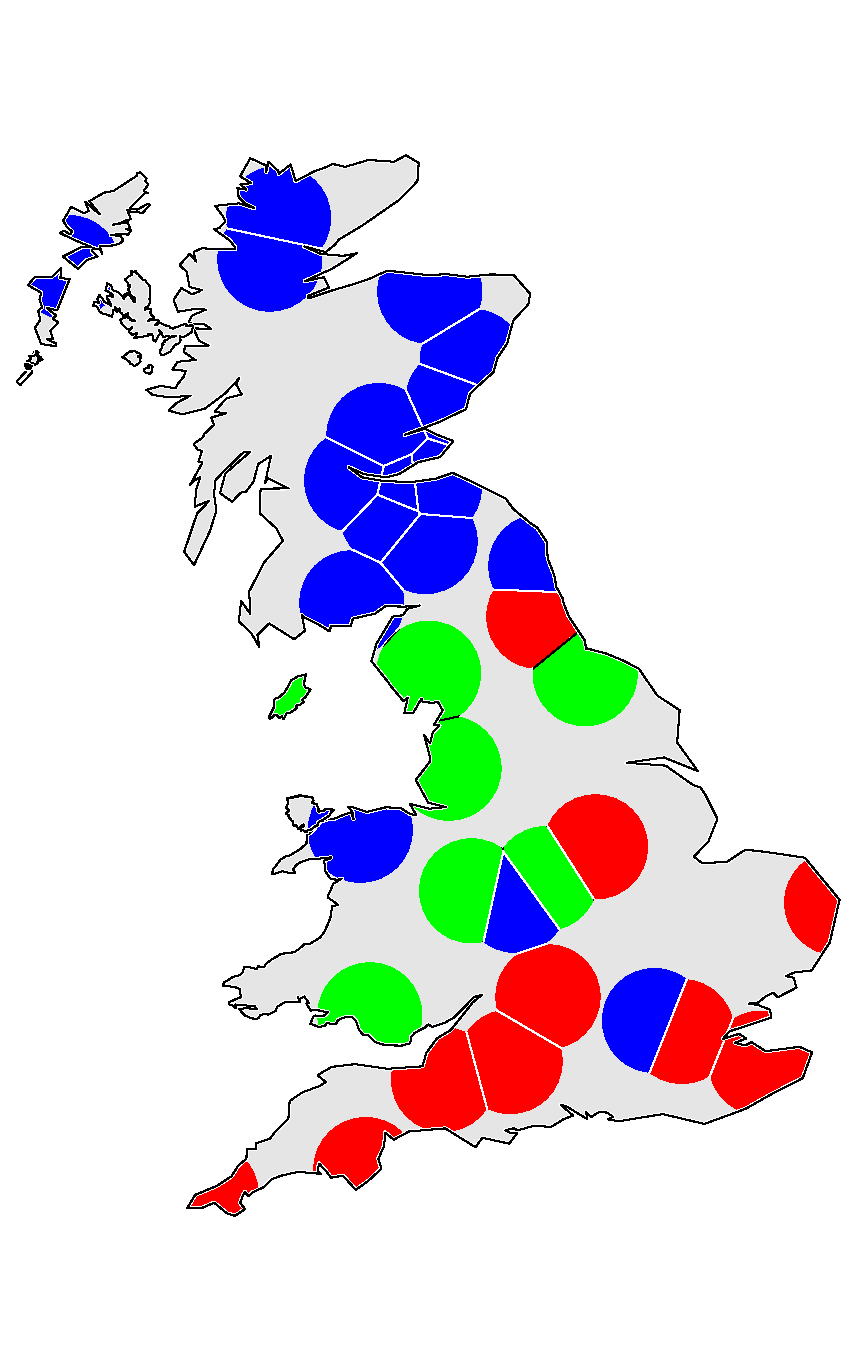
\includegraphics [keepaspectratio,width=.98\textwidth] {illustrations/wolk_WARD_lingdist_hard.eps}
\end{minipage}
\begin{minipage}[b]{0.30\linewidth}
    \centering
    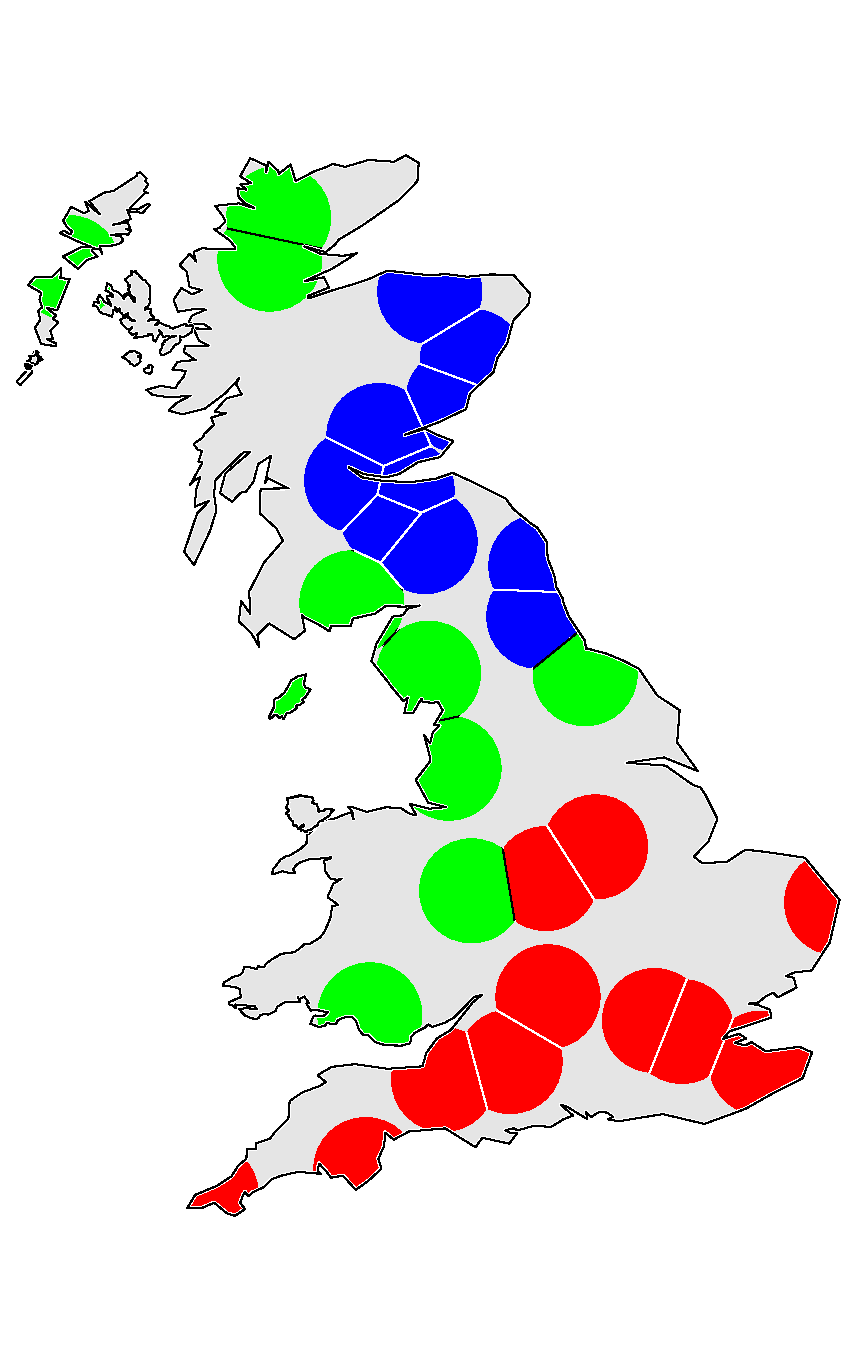
\includegraphics [keepaspectratio,width=.98\textwidth] {illustrations/wolk_noisy_cluster_gam_r2-3groups.eps}
\end{minipage}
\caption{Cluster maps -- hierarchical agglomerative cluster analysis (displayed: 3-cluster solution). Left: geographic as-the-crow-flies distances. Center: normalization-based morphosyntactic distances. See \citet[chapter 6]{szmrecsanyi_grammatical_2013} for details. Right: probabilistically enhanced morphosyntactic distances.} \label{clustermapsfig}
\end{sidewaysfigure}
%%%%%%%%%%%%%%%%%%%%%%%%%%%%%%%%%%%%%%%%%%%%%%%%%%%%%%%%%%%%%%%%%%%%%%%%%%%%%%%%%%%%%%%%%%%%%%%%%%%%%%%%%%%%%%%%%%%%%%%%%%%%%%%

In the left-hand and center maps of Figure \ref{clustermapsfig} we find two cluster maps that correlate (\citealt{goebl_dialectometrie_2005}) Great Britain's geographic landscape to its dialect landscape. For expository purposes, both maps display a 3-cluster solution, but we do not wish to claim that this is necessarily the optimal solution. The left-hand map clusters a distance matrix detailing not linguistic distances but as-the-crow-flies geographic distances between dialect sites, thus depicting, for reference purposes, a geographically maximally neatly partitioned map. This map suggests that on strictly geographic grounds, Great Britain can be partitioned into three coherent areas: a red region comprising  the South of England plus the county of Glamorganshire in Southern Wales; a green region containing the North of England plus the county of Denbighshire in Northern Wales plus the county of Dumfriesshire in Southern Scotland; and a blue region encompassing Scotland minus the county of Dumfriesshire.

Compare this scenario to the map in the center of Figure \ref{clustermapsfig}, which projects a corresponding regionalization on morphosyntactic grounds. There is a good deal of geographic incoherence in the morphosyntax division: For example, there are blue outliers all over England and Wales; Durham in the North of England is categorized as a red (i.e. Southern) county; Glamorganshire in Southern Wales is a green (i.e. Northern) county; and so on. That said, there is clearly some similarity between the geographic and linguistic partitioning, because the tripartite division between Scotland, the North of England, and the South of England is essentially in place. We conclude that our corpus-based measure of aggregate morphosyntactic variability does detect a geolinguistic signal.



\subsection{The probabilistically enhanced top-down \textsc{cbdm} approach}
\label{sec:prob}

While the signal discussed in the previous section seems to broadly match the description in the literature, it also raises some concerns.
First, the outliers are difficult to motivate.
Why should, for example, Middlesex group with Scotland?
For most of the outliers, individual significant differences to their geographically close neighbors can be found \citep[chapter 7]{szmrecsanyi_grammatical_2013}, but this does not sufficiently explain the cluster structure.
Second, the results do not confirm two of the most reliable results of the atlas-based dialectometric enterprise: both the shape and the strength of the relationship between linguistic and geographic distances are markedly different.
\citet{nerbonne_how_2013} summarizes several studies, finding that geographic distance (statistically) explains 16 to 37 percent of the variance in linguistic distance, and that the relationship is sublinear: as one considers location pairs that are further apart, the increase in linguistic dissimilarity begins to level off.
In contrast the corpus signal yields a very low correlation between linguistic and geographic (``as the crow flies'') distances, explaining only approximately 4.4 percent of the variance, and the relationship is linear rather than sub-linear.
Using travel time as the operationalization of geographic distance \citep{gooskens_traveling_2005} improves the relationship slightly to almost 8 percent; nevertheless, it is still far below what is typically found.
This suggests that some form of bias may exist in the data set.

It is a well-known effect that non-linguistic aspects of the data set and its creation can influence the aggregate results, such as the specific fieldworker covering a location \citep[``field worker isoglosses'', ][241ff.]{trudgill_contribution_1982}.
Similar problems may reside in the corpus at hand.
We suggest that one issue in particular causes a substantial amount of the divergences from the usual pattern: the fact that the amount of corpus material per county varies, and in some cases the number of words per county may be very small.
Measurements that are based on little data are imprecise, and so are the distances resulting from them.
We can test the influence of this factor by exploring the relationship between linguistic distance and an appropriate operationalization of corpus size (and therefore accuracy).

\begin{figure}[tbp]
\begin{minipage}[b]{0.45\linewidth} % A minipage that covers half the page
    \centering
    \vfill
    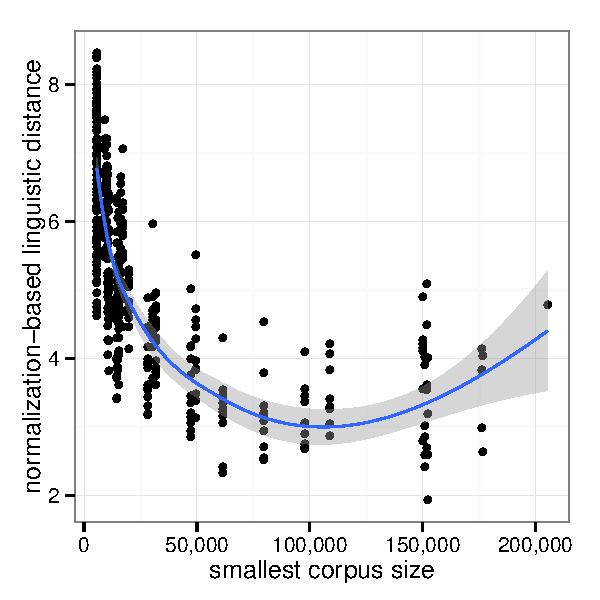
\includegraphics [keepaspectratio,width=.98 \textwidth] {illustrations/wolk_min-norm.pdf}
    \vfill
\end{minipage}
\hspace{0.5cm} % To get a little bit of space between the figures
\begin{minipage}[b]{0.45\linewidth}
    \centering
    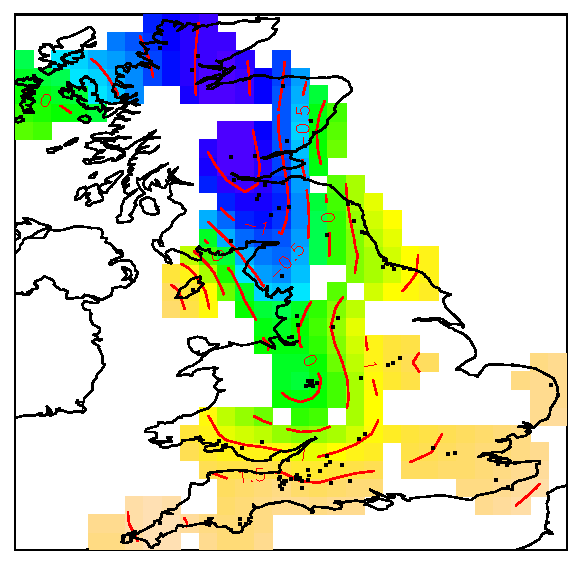
\includegraphics [keepaspectratio,width=.98\textwidth] {illustrations/wolk_multneg-gam.pdf}
\end{minipage}
\caption{Left: Correlation of minimum subcorpus size and linguistic distance (top down normalization-based approach; $R^2=0.61$) Right: Example \textsc{gam} for multiple negation (log scale). Lighter colors indicate higher frequency. Red lines indicate shape of the frequency gradient.} \label{fig:cor-ling}
\end{figure}


The left-hand part of Figure \ref{fig:cor-ling} displays the linguistic distance between county pairings as a function of the smaller of the two subcorpus sizes; a smoother line is included to highlight the general trend.
Clearly, there is a strong relationship: distances involving the counties with the worst coverage are consistently too high. 
At approximately 50,000 words, this relationship largely levels off\footnote{The small uptick at the end is a combination of data sparsity (due to the small number of subcorpora of that size) and the somewhat atypical, but large Suffolk subcorpus.}.
The outliers in Figure \ref{clustermapsfig} fall below this threshold: for example, the subcorpus for Durham consists of 28,000 words, and that for Middlesex of 32,000.
These three measures of quality -- interpretability of groupings, correlation with geography, and influence of the amount of data -- suggest that there may be a bias in the data that obscures the pattern.
Note, however, that these measures serve more as ``sanity checks''\footnote{We thank an anonymous reviewer for this phrasing.} than as proper external validation.
A method that fares better under this yardstick is not necessarily correct, but a method that fares worse indicates potential problems.

We therefore propose to use some form of smoothing that takes the accuracy of the measurement into account.
Per the Fundamental Dialectological Postulate \citep{nerbonne_toward_2007}, geographic smoothing seems particularly appropriate: in the absence of compelling evidence to the contrary, we should assume that proximate varieties resemble each other.
Several methods of doing such smoothing have been proposed, including intensity estimation \citep{rumpf_structural_2009}, local spatial autocorrelation \citep{grieve_corpus-based_2009}, and generalized additive models \citep[\textsc{gam}s;][]{wieling_quantitative_2012}.
We believe that \textsc{gam}s are an especially adequate choice, as they are a variant of regression modeling, and therefore closely resemble the techniques in common use by, among others, variationist sociolinguists \citep{tagliamonte_variationist_2012}.
Using such models, it is possible to account for other factors that may influence the result, whether language-internal (e.g. subject type) or -external (e.g. speaker age).
In \citet{wolk_integrating_2014}, two language-external factors were included, namely speaker age and gender\footnote{As the relevant information was missing for a small number of texts (including all texts from three counties, see Section \ref{FRED}), they had to be removed from the analysis.}.
We keep these two factors for the analysis presented here, to account for any imbalances in the corpus sampling process.
For many features, there are significant effects of these factors, largely in the expected direction (i.e. female speakers use fewer non-standard features and older speakers use more archaic features).
Simulations based on these results, however, suggest that the overall effect that the inclusion of these factors has on the resulting distances is marginal \citep[233f.]{wolk_integrating_2014}.


In contrast to the GAM-based method used in \citet{wieling_quantitative_2012}, \citet{wolk_integrating_2014} did not model the distances directly, but built a separate model for each feature.
Furthermore, features that represent binary alternations\footnote{The selection of features to model as alternations was based on the variationist literature and on certain features existing as standard/non-standard variants in the original list.}, such as habitual \emph{would} vs. \emph{used to} or \emph{will} vs \emph{going to} as future markers, were modeled as such, rather than as individual frequencies.
Doing so removes potential bias resulting from base rate differences (e.g. differing frequencies of habitual or future contexts regardless of form) between speakers/counties, and makes the results more comparable to variationist research on these features, which typically utilizes \textsc{varbrul}-style modeling.
This yields a list of 45 remaining features, and therefore the number of models included in the analysis is also 45.
Each model contains a two-dimensional geographic smoother that allows the feature to vary by location in a gradient fashion.
An example for this can be seen in the right-hand map in Figure \ref{fig:cor-ling}, displaying the smoother for multiple negation.
As expected, the feature is rare in Scotland and relatively frequent in the South of England, with the North forming a transition zone.
This model is then used to predict the proportion of one realization, or the frequency to be expected in ten thousand words.
From here on, the analysis proceeds as outlined above.

A cluster map of the resulting distances is presented in the right-hand part of Figure \ref{clustermapsfig}. 
The tripartite division remains, and the large-scale areas are geographically coherent, with the exception of the young dialects in the Scottish Highlands and the Hebrides, which group with the North of England.
Quantitatively, the model fares well: The relationship between geographic and linguistic distances is sublinear and solid ($R^2 = 0.44$ for least-cost travel time; compare the normalization-based value of $0.08$).
Even more importantly, the influence of subcorpus size has greatly decreased and now accounts for only 16.2 percent of the variance, compared to 61 percent for the normalization-based distances.

We hasten to add that this clean pattern is hardly surprising: the \textsc{gam}s have geographic coherence built into their assumptions. 
Therefore, it can be argued that the results may be too homogeneous, that there are true differences that the \textsc{gam}s smooth over.
Nevertheless, the model produces at least an upper boundary for spatial cohesion; and a bias in favor of the Fundamental Dialectological Postulate seems more plausible than a bias toward accidental properties of the corpus compilation process.
Furthermore, the resulting association between geography and linguistic distance, while on the high side, is not outside the range of what one would expect based on traditional dialectometric analyses.
It is also clearly distinct from $1$, indicating that there is still unpredictable dialectal variation left.
Finally, it bears noting that the \textsc{gam} process yields interpretable single feature maps as a byproduct -- a rather beneficial property of this approach.

\section{Bottom-up CBDM} \label{bottomup}

So far, we have covered methods that rely on a pre-specified feature list.
In the following, we explore whether it is possible to eliminate such a list and go directly from the corpus to a distance measurement.
Directly measuring corpus (dis)similarity is an important, yet somewhat underresearched, topic in corpus linguistics \citep{kilgarriff_comparing_2001}.
This is especially true for morphosyntactic measures\footnote{\citet{scherrer_recovering_2012} provides a method for deriving pronunciation distances between corpora automatically, but this approach is not straightforwardly generalizable to morphosyntax,}.
The method proposed here builds on an idea proposed by \citet{nerbonne_measure_2006}, who employ part-of-speech n-grams to compare syntactic differences between two corpora.
The method makes use of permutation tests to determine how reliable frequency differences between the corpora are, a technique that is gaining popularity in corpus linguistics \citep{lijffijt_computational_2013}.
The first full dialectometric use of such an approach was by \citet{sanders_statistical_2010}, who used it to explore a Swedish dialect corpus.
Let us exemplify the general idea starting with comparisons between county pairs.

Consider the following utterance from the Devon subcorpus of \textsc{fred-s}:

\begin{exe}
\ex We\textsubscript{\texttt{PPIS2}} started\textsubscript{\texttt{VVD}} at\textsubscript{\texttt{II}} three\textsubscript{\texttt{MC}} ,\textsubscript{\texttt{,}} yes\textsubscript{\texttt{UH}} .\textsubscript{\texttt{.}}  <DEV\_005>
\end{exe}

Ignoring punctuation, we construct all overlapping sequences of length $n$ (here, always $n=2$, i.e, \emph{bigrams}), yielding the following result: \textsc{ppis2\_vvdi}, \textsc{vvd\_ii}, \textsc{ii\_mc}, \textsc{mc\_uh}. 
This is done for all utterances in both subcorpora, and the resulting bigram counts are aggregated on the county level.
A normalization procedure that redistributes probability point mass is applied to the resulting absolute frequencies.
More specifically, this normalization process keeps the total number of tokens per n-gram constant, but scales the per-county numbers according to the amount of n-grams in that county\footnote{This method was chosen based on the process described in \citet{nerbonne_measure_2006}.
The difference to a more familiar normalization scheme seems to be marginal -- the correlation between raw distances derived using this method and those from simple per 10,000 n-grams normalization is greater than $0.99$.}.
Then, the data is randomly resampled (without replacement) based on turns\footnote{\citet{nerbonne_measure_2006} resample based on sentences; in later work \citep{wiersma_automatically_2011}, this was changed to resampling based on speakers to increase the reliability of the result.
This was not feasible for this study, as the number of speakers for some of the counties was low \citep[see also][]{sanders_statistical_2010}.}
and the procedure is repeated on the new corpus.
In other words, a new corpus is created, in which each county subcorpus contains the same amount of turns, but each turn is randomly assigned to a county.
We can now, for each n-gram, calculate the difference in normalized values between the two counties both in the ``true'' (i.e. original) corpus and the randomly resampled one.
If this difference is smaller in the original corpus, we can count this as evidence that the original difference may have occurred purely by chance - after all, a random process yielded a greater difference.
Finding that the difference for the permuted corpus is smaller, however, would be consistent with the hypothesis that there is a genuine difference between the counties.
If this process is not only done once, but a large number of times, the proportion of cases where the original difference was actually greater yields a probabilistic measure of how significant a n-gram frequency difference between the two counties is.
In a similar fashion, the overall distance (computed using a suitable distance metric, such as the Manhattan distance) can be evaluated.

In addition, we can run the permutation not only on county pairs, but over all counties at the same time.
Instead of comparing differences between counties, we calculate the proportion of random corpora in which the normalized frequency exceeds that of the true corpus, counting runs where they are equal as one half.
This yields a \emph{reliability matrix} that indicates how reliably this n-gram appears more (or less) frequently than expected by chance.
Using either the pairwise number of significant differences or a measure of the extremeness of the distribution derived from the reliability matrix, we can evaluate particularly distinctive patterns.
For example, consider \texttt{AT\_NN1}, the definite article followed by a singular noun, the most frequent pattern.
This pattern was significantly different in 84 of all the 136 possible pairwise county combinations; this amounts to being the 29th most distinct n-gram according to this metric,
If, on the other hand, we use the number of divergences per n-gram from maximally consistent whole-corpus permutations, we obtain a value of 2.42 percent.
This is still one of the top patterns, but ranks quite a bit lower at number 83 on the corresponding list.
In general, a similar pattern seems to hold: there is a strong correlation between the two measures of distinctiveness, but the number of pairwise significant differences is more strongly influenced by n-gram frequency.
Both the normalized frequency matrix and the reliability matrix are suitable for distance calculations.
Details about the process can be found in \citet[64-74]{wolk_integrating_2014}.

\begin{sidewaysfigure}[tbp]
\begin{minipage}[b]{0.30\linewidth} % A minipage that covers half the page
    \centering
    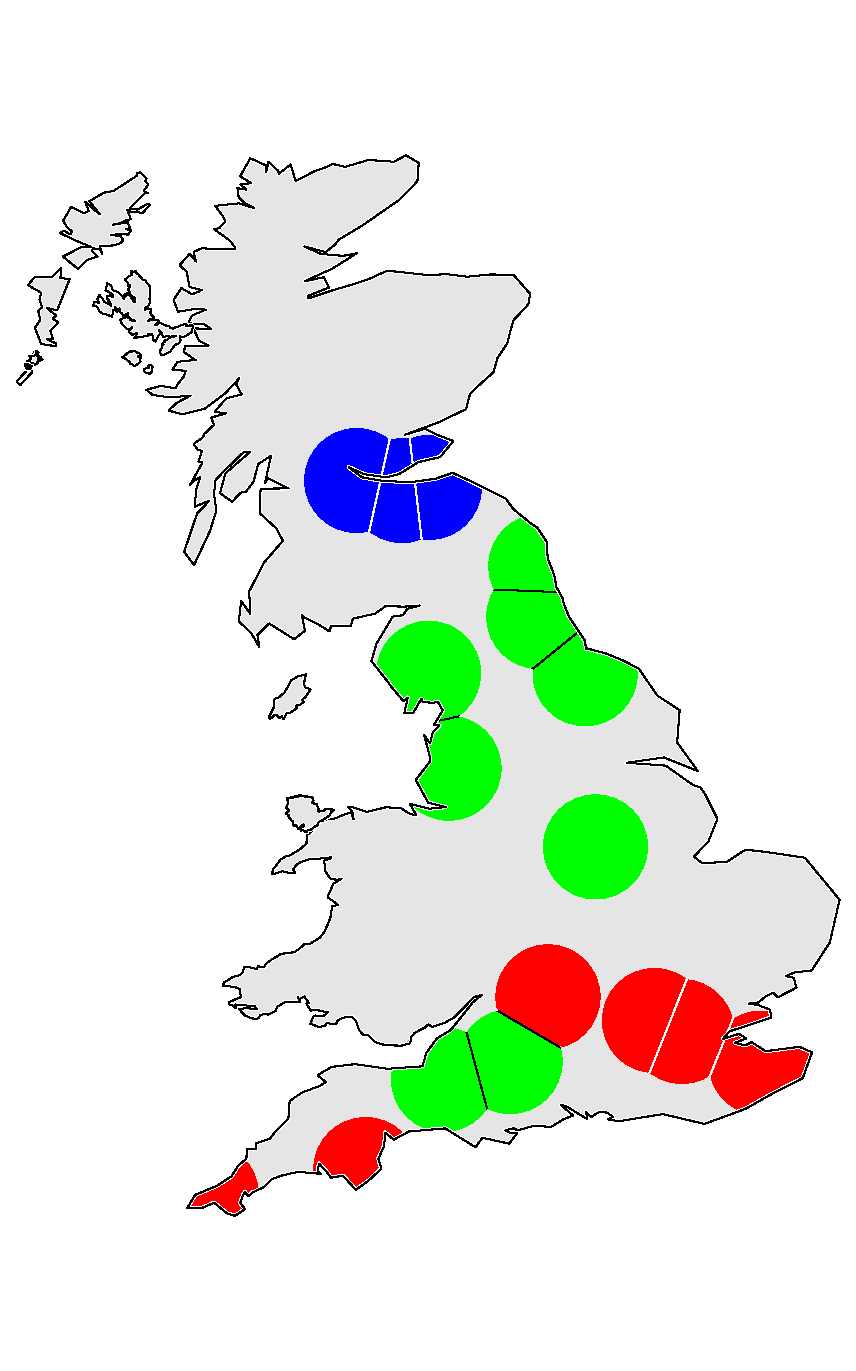
\includegraphics [keepaspectratio,width=.98\textwidth] {illustrations/wolk_noisy_cluster_normalized_fredS-3groups.eps}
\end{minipage}
%\hspace{0.5cm} % To get a little bit of space between the figures
\begin{minipage}[b]{0.30\linewidth} % A minipage that covers half the page_reference_to_a_page
    \centering
    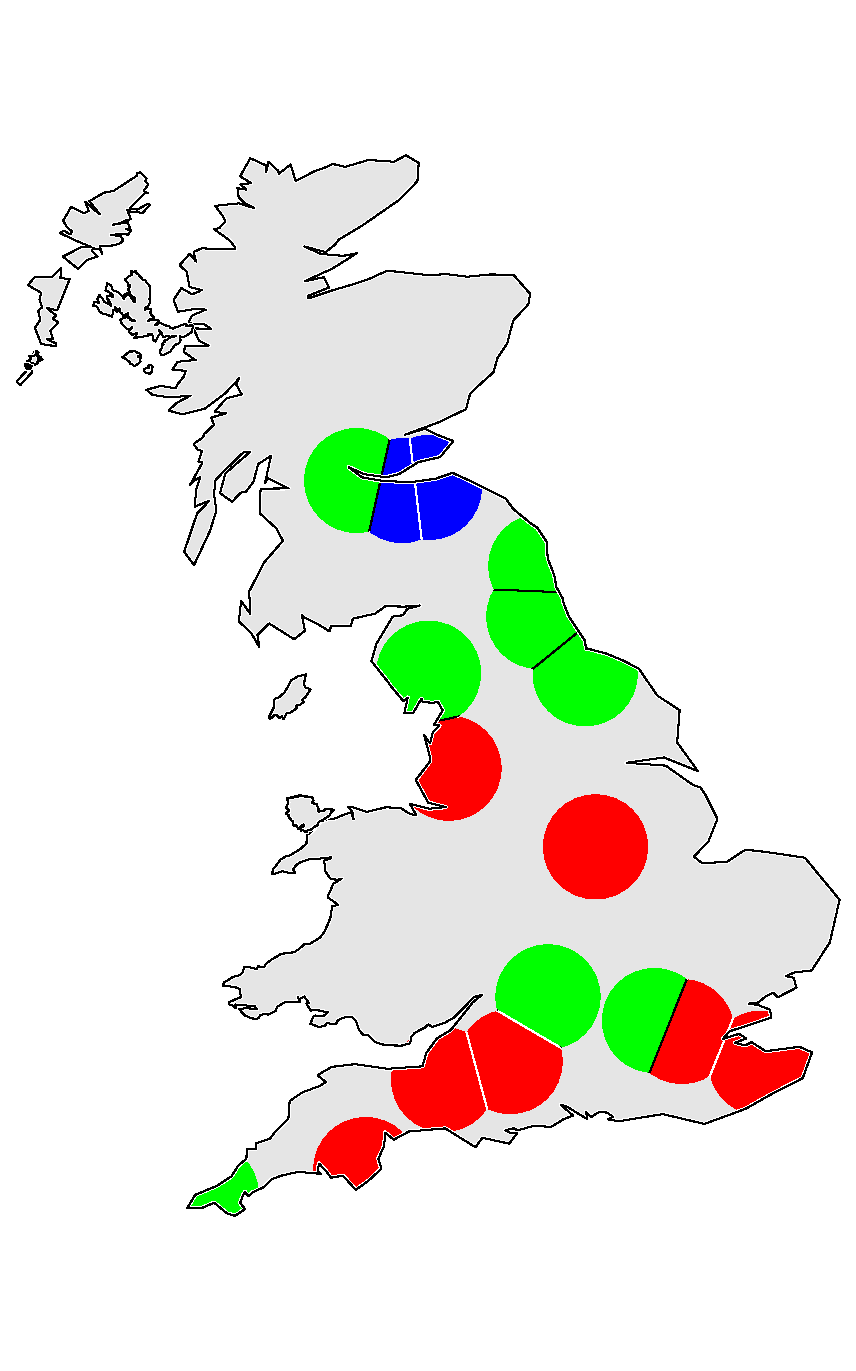
\includegraphics [keepaspectratio,width=.98\textwidth] {illustrations/wolk_noisy_cluster_frequency-3groups.eps}
\end{minipage}
\begin{minipage}[b]{0.30\linewidth}
    \centering
    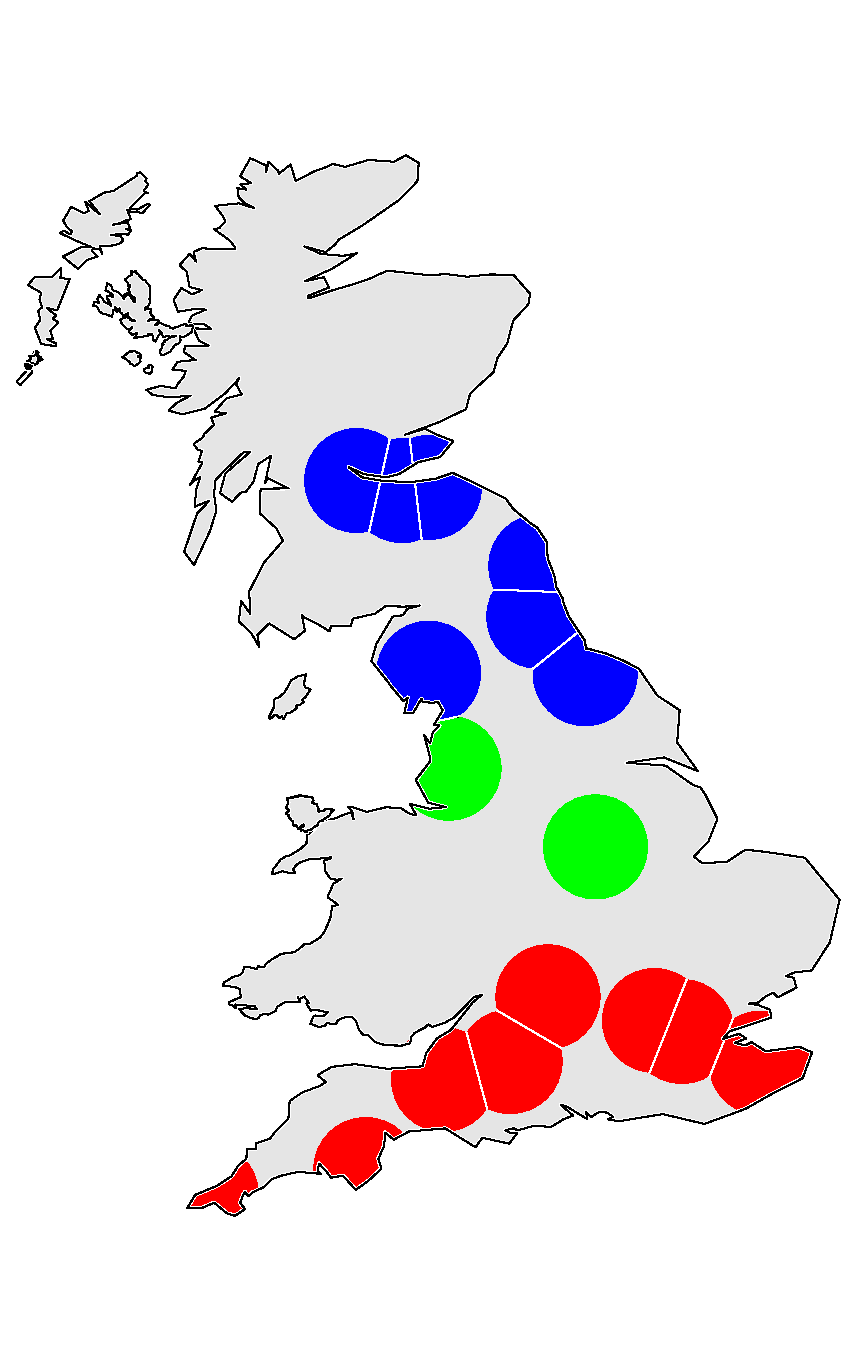
\includegraphics [keepaspectratio,width=.98\textwidth] {illustrations/wolk_noisy_cluster_reli7-3groups.eps}
\end{minipage}
\caption{Cluster maps -- hierarchical agglomerative cluster analysis using Ward's method as clustering algorithm (displayed: 3-cluster solution). Left: Top-down normalization-based approach on \textsc{fred-s}. Center: Bottom-up normalized frequencies. Right: Bottom-up reliability scores.} \label{fig:bup-maps}

\end{sidewaysfigure}

Figure \ref{fig:bup-maps} displays the results.
For comparison, the left-hand map displays the results of the normalization-based\footnote{This comparison is more appropriate than that to the model-based variant, as both do not employ geographic smoothing.} top-down approach on the texts that are available in \textsc{fred-s}.
First, we note that the approach fares better here than on the complete data set: the clusters are spatially mostly coherent, geographic distance explains 27.6 percent of the variance in linguistic distances, and text size differences account for a slightly lower share of 48.5 percent. 
This results from the removal of most counties with particularly restricted textual coverage.
The center map, showing a cluster analysis of normalized bottom-up frequencies, yields a much messier picture; moreover the quantitative match of the linguistic distances is considerably worse: the $R^2$ for geographic distances is much lower at 0.10, and that for text size considerably higher at a staggering 0.67.
The right plot, finally, shows the clusters resulting from the reliability matrix, restricted to bigrams with at least seven pairwise significant differences.
Here, the match between geographic and linguistic distances is almost as good as for the top-down result on the left at 26.2 percent, and the influence of corpus size is significantly lower ($R^2 = 0.16$).
Qualitatively, we find that contiguous regions emerge. 
This analysis finds a division between Scotland and the North of England only at a position of lower importance, and instead emphasizes a transition area between the North and South of England.
Finally, we add that both measures of distinctiveness identify dialectologically meaningful patterns.
Among the ten most distinctive n-grams, for example, we find many known features of British dialect grammar: several bigrams related to \emph{was/were} variation (\textsc{pph1/pphs1/pphs2\_vbdr}, \emph{it/(he/she)/they were}, and \textsc{pphs2\_vbdz}, \emph{they was}), \emph{them} as a determiner (in particular after temporal nouns, as in \emph{them days}), \emph{used to} as a marker of habituality (in particular following nouns), and \emph{is n't/not}, which competes with the non-standard form \emph{ain't}.

In short, then, our results suggest that bottom-up \textsc{cbdm} is practicable and worthwhile; the best method yielded results comparable to those for the manually selected feature set. 
The normalized frequencies, however, fared rather badly, and only after the permutation process smoothed off the rough edges did the areal signal emerge.

Finally, it bears mentioning that the nature of the tag set and the tagging procedure used have a strong influence on the linguistic patterns that emerge, and therefore most probably also on the aggregational results.
Exploring the effect of changes in the data pipeline will be crucial in the further development of this approach.

\section{Conclusion} \label{conclusion}

In this contribution, we have sketched some recent advances in corpus-based dialectometry (\textsc{cbdm}).
\textsc{cbdm} bases claims about geolinguistic patterns in aggregate linguistic variability on language usage as observed through naturalistic corpus data (as opposed to e.g. linguistic knowledge).
Early studies in \textsc{cbdm} (e.g. \citealt{szmrecsanyi_corpus-based_2011}) aggregate normalized text frequencies of features in an a-prioristically defined feature catalogue.
This approach we have called the normalization-based top-down \textsc{cbdm} approach (see Section \ref{topdownnormalized}).
What we have shown is that top-down \textsc{cbdm} profits from the probabilistic modeling of usage frequencies prior to aggregation.
The other major advance we have dwelt on in this contribution is bottom-up \textsc{cbdm}, which does not draw on a pre-defined feature catalogue but lets the features to be aggregated emerge in a data-driven fashion through the identification of significant and/or distinctive part-of-speech \emph{n}-grams.
Both probabilistically enhanced top-down \textsc{cbdm} and bottom-up \textsc{cbdm} are valuable additions to the dialectometry toolbox.

With regard to the theme of the present volume, ``The Future of Dialects'', we have discussed in this contribution new ways of analyzing dialect data.
These new ways are in line with usage-based methodologies customary in related disciplines such as variationist sociolinguistics. 
As we have argued in the Introduction section, we believe that the future of dialectology will crucially include the ability to analyze actual usage data. 
As for the future of dialects \textit{per se}, we would like to stress that a focus on more realistic, usage-oriented data sources is likely to reflect the many-faceted nature of dialects more faithfully than other methodologies do. 

\section*{Acknowledgments}

We wish to thank Peter Kleiweg for creating and maintaining the RuG/L04 package. The audience at the Workshop on 'Frontiers in the study of language variety' at the Methods XV conference in Groningen (August 2014) provided very helpful and valuable feedback on an earlier version of this paper. We also thank three anonymous reviewers for their extensive and constructive feedback. The second-named author gratefully acknowledges an Odysseus grant awarded by the Research Foundation Flanders (FWO, grant no. G.0C59.13N). The usual disclaimers apply.


%\printbibliography[heading=subbibliography,notkeyword=this]
% The following inserted by BS
%\bibliography{diam}
\il{British English|)}

\printbibliography[heading=subbibliography,notkeyword=this]
\end{document}
